\chapter{Simulation results}\label{ch:simulationResults}

\section{Playground definition}\label{ch:3DPlaygroundDefinition}
\noindent For purpose of testing, new playground (\ref{fig:new3DPlayground})with added dimension needs to be introduced. Additional element of \textit{mission control} needs to be introduced, because previous experiments was with not coordinated flight and for real missions some coordinated flight is required, therefore waypoint set $\mathscr{WP}$ is added into playground. 
\begin{figure}[H]
    \centering
    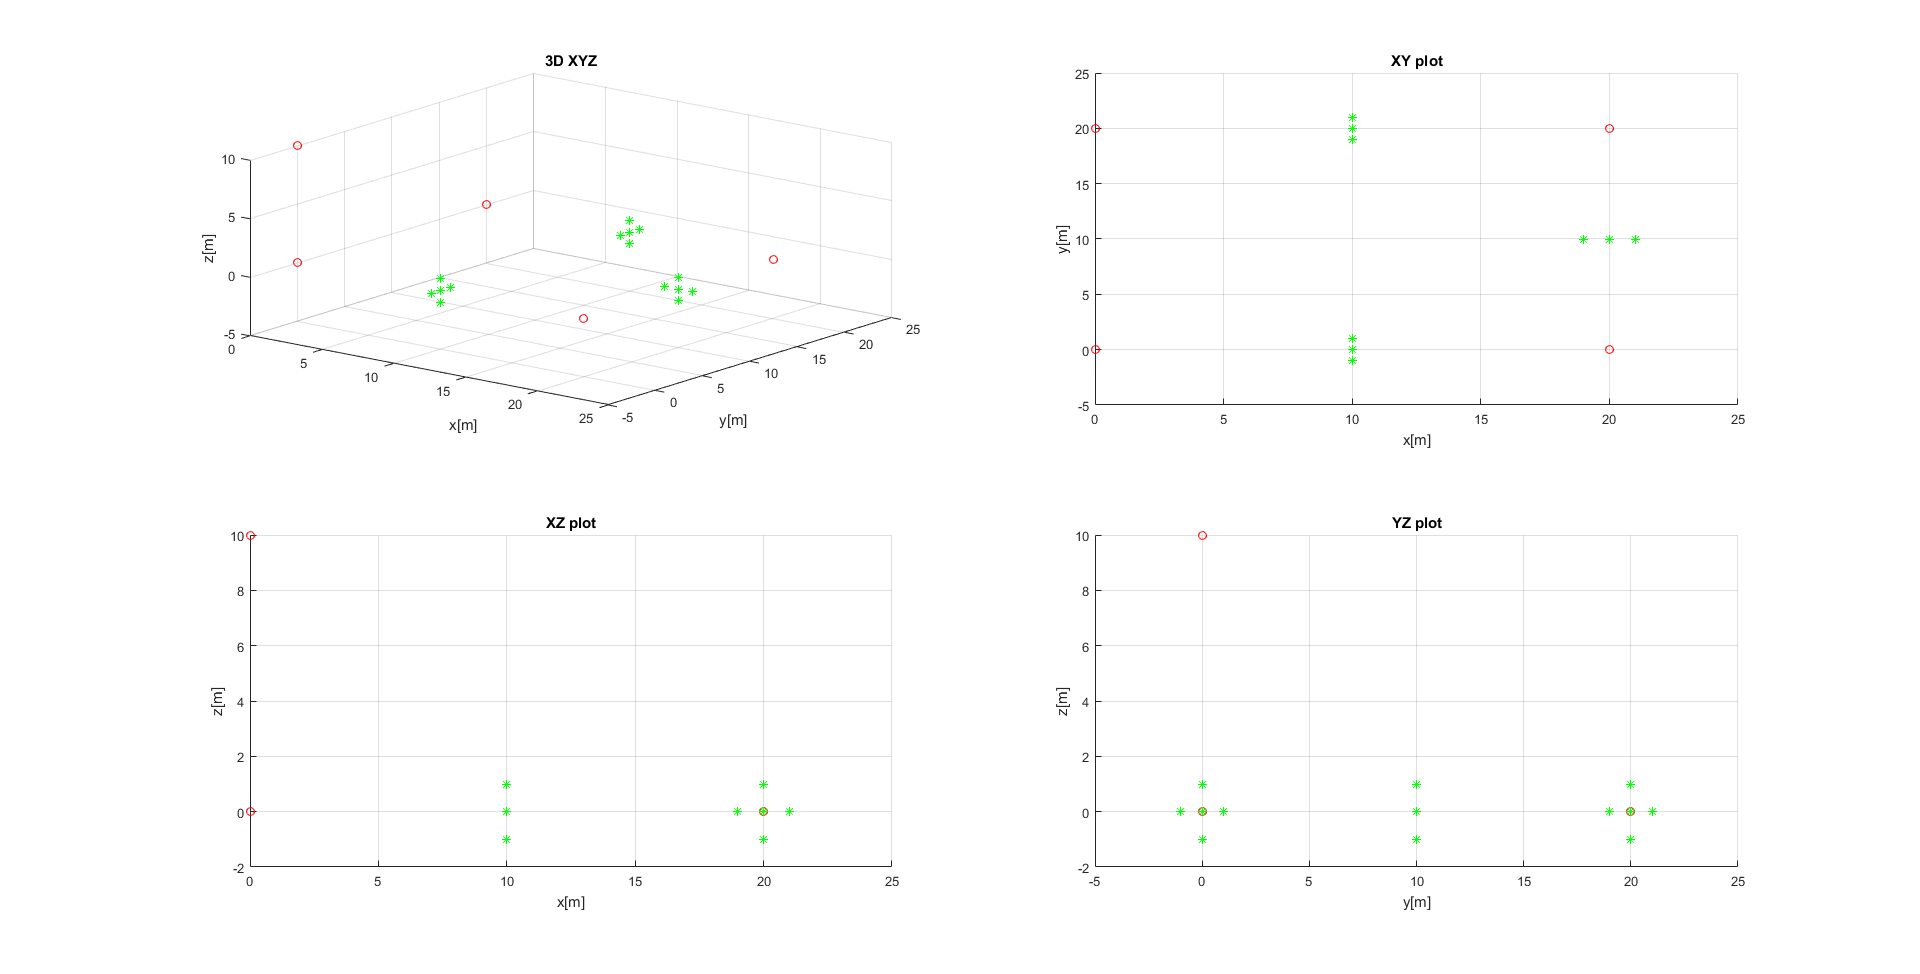
\includegraphics[width=\linewidth]{\FIGDIR/37_Playground_3D.png}
    \caption{Initial playground for obstacle avoidance and optimal path finding testing}
    \label{fig:new3DPlayground}
\end{figure}
\noindent Waypoint set $\mathscr{WP}$ (\ref{eq:playground3DSimpleWPSet}) contains five waypoins in Cartesian coordinates $\mathscr{WP}_i =[x,y,z]^T$. This set is simple rectangular flight around rectangle with side of 20 meters and slightly elevated end by 10 meters $\mathscr{WP}_E$.

\begin{equation}\label{eq:playground3DSimpleWPSet}
    \begin{aligned}
          \mathscr{WP} = \{ \mathscr{WP}_S &=[0,0,0]^T,\\
                            \mathscr{WP}_1 &=[20,0,0]^T,
                            \mathscr{WP}_2 =[20,20,0]^T,\\
                            \mathscr{WP}_3 &=[0,20,0]^T,
                            \mathscr{WP}_E =[0,0,10]^T,\}
    \end{aligned}
\end{equation}
\newpage 
\noindent Each path tracking algorithm needs to have stop condition which indicates when vehicle should stop following presented waypoint. Usually unit ball stop condition is used (\ref{eq:stopFunctionUnitBall}) where $[x_v,y_v,z_v]^t$ is vehicle position, $[x_g,y_g,z_g]^T$ is waypoint position and $p_t$ is precision threshold.
\begin{equation}\label{eq:stopFunctionUnitBall}
    \norm{\begin{bmatrix}x_g-x_v\\y_g-y_v\\z_g-z_v\end{bmatrix}} \le p_t
\end{equation}
Single obstacle $o_i\in\mathscr{O}$ is defined by its position $o=[x_o,y_o,z_o]^T$. All obstacles are stored in single obstacle structure $\mathscr{O}$ defined by (\ref{eq:3dSimplisticPlaygroundO}).
\begin{equation}\label{eq:3dSimplisticPlaygroundO}
    \mathscr{O} = \{\mathscr{O}_1,\mathscr{O}_2,\mathscr{O}_3\}
\end{equation}
Obstacle subset $\mathscr{O}_1$ (\ref{eq:3dSimplisticPlaygroundO1}) is defined between waypoints $\mathscr{WP}_S,\mathscr{WP}_1$.
\begin{equation}\label{eq:3dSimplisticPlaygroundO1}
    \mathscr{O}_1 = \{[10,0,0]^T,[10,1,0]^T,[10,-1,0]^T,[10,0,1]^T,[10,0,-1]^T\}
\end{equation}
Obstacle subset $\mathscr{O}_2$ (\ref{eq:3dSimplisticPlaygroundO2}) is defined between waypoints $\mathscr{WP}_1,\mathscr{WP}_2$.
\begin{equation}\label{eq:3dSimplisticPlaygroundO2}
    \mathscr{O}_2 = \{[20,10,0]^T,[20,10,1]^T,[20,10,-1]^T,[19,10,0]^T,[21,10,0]^T\}
\end{equation}
Obstacle subset $\mathscr{O}_3$ (\ref{eq:3dSimplisticPlaygroundO3}) is defined between waypoints $\mathscr{WP}_2,\mathscr{WP}_3$.
\begin{equation}\label{eq:3dSimplisticPlaygroundO3}
    \mathscr{O}_3 = \{[10,20,0]^T,[10,20,1]^T,[10,20,-1]^T,[10,19,0]^T,[10,21,0]^T\}
\end{equation}

\section{Movement automaton predictor}\label{ch:movementAutomatonPredictor}
\noindent Vehicle system is given by model from section \ref{sec:3DsimplisticplaneModel}. Vehicle control is defined as movement automation $\mathscr{MA}$ with rapid exploration movement set defined in equation \ref{eq:rapidExplorationMovementSet}. Movement predictor needs to be developed in order to obtain control signal $u(t)$ It is possible to predict movement buffer $B_{\mathscr{MA}}$, between vehicle initial position $x_0$ and waypoint, when known obstacle set $\mathscr{O}$ is given and movement state can be predicted for chain of movements. This approach have been defined in alg. \ref{alg:05}. as rapid exploration tree. 

Vehicle state $x(t_0)$ at start of mission execution is known. Vehicle state in discrete time $x(t)$ is given by equation \ref{eq:vehicleStateDiscreteKnown}. Where $x_v(t),y_v(t),z_v(t)$ is vehicle position in local coordinate frame and $\alpha_v(t),\beta_v(t),\gamma_v(t)$ is vehicle orientation angles.
\begin{equation}\label{eq:vehicleStateDiscreteKnown}
    x(t) = [x_v(t),y_v(t),z_v(t),\alpha_v(t),\beta_v(t),\gamma_v(t)]^T;
\end{equation}
Base movement table for movements $m_i(1)\in M$ have been measured on system model (\ref{sec:3DsimplisticplaneModel}). This table represents vehicle position and orientation differences after execution of movement. Vehicle initial state was set at center of local coordinate frame with narrow orientation $[x_0,y_0,z_0]=[0,0,0]$. Vehicle initial orientation was aligned with main frame axis X, therefore initial orientation angles are $[\alpha_0,\beta_0,\gamma_0] = [0,0,0]$. Vehicle velocity was set to constant value $v_v = 1 ms^{-1}$. Vehicle position after movement execution is given by parameters $x_b,y_b,z_b$ at time $t+1$. Vehicle orientation is given by parameters $\alpha_b,\beta_b,\gamma_b$. Givem parameters are also absolute shifting, because initial state is $[x_0,y_0,z_0,\alpha_b,\beta_b,\gamma_b]$ set to $\vec{0}$.
\begin{table}[H]
    \centering
    \begin{tabular}{|l||c|c|c|c|c|}
    \hline
        $v_x/m_i$           &    Straight $\circledcirc$ & Down $\Downarrow$  & Up $\Uparrow$    & Left $\Leftarrow$ & Right $\Rightarrow$\\\hline\hline
        $x_b [m]$           &    1.00	  & 0.98  & 0.98  & 0.98 & 0.98\\\hline
        $y_b [m]$           &    0	      & 0	  & 0	  & 0.13 & -0.13\\\hline
        $z_b [m]$           &    0	      & -0.13 & 0.13  &	0	 & 0\\\hline
        $\alpha_b [rad]$	&    0	      & 0	  & 0	  & 0    & 0\\\hline
        $\beta_b [rad]$     &    0	      & 0.2   & -0.26 & 0	 & 0\\\hline
        $\gamma_b [rad]$    &    0	      & 0	  & 0	  & 0.26 & -0.26\\\hline
    \end{tabular}
    \caption{Base values for movement application, vehicle position difference $x_v,y_v,z_v$ and orientation differences $\alpha_v,\beta_v,\gamma_v$.}
    \label{tab:movementPredictor}
\end{table}
\noindent With defined base movement table (tab. \ref{tab:movementPredictor}). with defined shifting for movement at time $t_0+1$, \textit{rotation} (\ref{eq:rotationSimplisticPredictor}) and \textit{shifting} (\ref{eq:shiftingSimplisticPredictor}) equations must be defined in order to obtain predicted position $\hat{x}(t+1)$. Position after movement execution $[\hat{x}(t+1),\hat{y}(t+1),\hat{z}(t+1)]$ is depending on vehicle orientation before movement execution $[\alpha_v(t),\beta_v(t),\gamma_v(t)]$. Rotation function rotates vehicle position $[x_b(t_0),y_b(t_0),z_b(t_0)]$ according to vehicle orientation angles $[\alpha_v(t),\beta_v(t),\gamma_v(t)]$. For rotation standard rotation matrix $R_{XYZ}(\alpha,\beta\gamma)$ (\ref{eq:xyzspaceRotationMatrix}) is used. Final position offset vector $[\tilde{x}_b(t+1),\tilde{y}_b(t+1),\tilde{z}_b(t+1)]$ at predicted time $t+1$ is given by equation \ref{eq:rotationSimplisticPredictor}.
\begin{equation}\label{eq:rotationSimplisticPredictor}
    \begin{bmatrix}
        \tilde{x}_b\\ 
        \tilde{y}_b\\
        \tilde{z}_b\\
    \end{bmatrix}
    = R_{XYZ}(\alpha_v(t),\beta_v(t),\gamma_v(t))
    \begin{bmatrix}
        x_b\\ 
        y_b\\
        z_b\\
    \end{bmatrix}
\end{equation}
Predicted state vector $\hat{x}(t+1)$ a at time $t+1$ is obtained by combining position offset vector $[\tilde{x}_b(t+1),\tilde{y}_b(t+1),\tilde{z}_b(t+1)]$, orientation offset vector $\alpha_b(t+1),\beta_b(t+1),\gamma_b(t+1)$. as given in equation \ref{eq:shiftingSimplisticPredictor}.\\
\begin{equation}\label{eq:shiftingSimplisticPredictor}
    \begin{aligned}
    \hat{x}(t+1) & = [\hat{x}_v(t+1),\hat{y}_v(t+1),\hat{z}_v(t+1),\hat{\alpha}_v(t+1),\hat{\beta}_v(t),\hat{\gamma}_v(t)]^T\\
    \hat{x}_v(t+1) & = x_v(t)+\tilde{x}_b\\
    \hat{y}_v(t+1) & = y_v(t)+\tilde{y}_b\\
    \hat{z}_v(t+1) & = z_v(t)+\tilde{z}_b\\
    \hat{\alpha}_v(t+1) & = \alpha_v(t) + \alpha_b\\
    \hat{\beta}_v(t+1) & = \beta_v(t) + \beta_b\\
    \hat{\gamma}_v(t+1) & = \gamma_v(t) + \gamma_b
    \end{aligned}
\end{equation}
Movement automaton $\mathscr{MA}$ has chaining property, therefore movement prediction chaining is also possible via recursive procedure for discrete execution time $t_i$. There exist predicted movement buffer $\hat{B}$ with ordered movement sequence $m_1(1),\dots,m_i(1)$, vehicle state after applying movement $m_{i+1}$ at time $t_i$ can be obtained via equation \ref{eq:discretePredictionChaining}.
\begin{equation}\label{eq:discretePredictionChaining}
    \hat{x}(t_i+1) = f(\hat{x}(t_i),m_{i+1}(1))
\end{equation}
Prediction function $f(\hat{x}(t_i),m_{i+1}(1))$ is in this case function defined by equation \ref{eq:shiftingSimplisticPredictor}, where parameters $[x_b,y_b,z_b,\alpha_b,\beta_b\gamma_b]$ are selected based on movement $m_{i+1}(1)$ type from lookup table  \ref{tab:movementPredictor}.


\section{Obstacle avoidance in partially known environment}
\noindent Obstacle avoidance is different in partially known environment, because uncertainty plays great role in control and decision making. Future obstacle avoidance theorem will be developed. Avoidance implementation have been verified at playground defined in section \ref{ch:3DPlaygroundDefinition}. Known world $\mathscr{F}$ have been mentioned multiple times over thesis. In case of reactive obstacle avoidance it is necessary to acknowledge that know world $\mathscr{F}$ is equal to $\mathscr{G}_{3D}$. Most of the time visible space (def. \ref{def:VisibleSpace}) is equal to visibility grid (def. \ref{def:visibilityGridCell}). Let say that for each discrete scanning time $t_i$ there exist avoidance grid $\mathscr{A}(t_i)$ which is valid for time $t\in[t_i,t_i+\tau)$, where $\tau$ is life time of scanned data. In real situation is frame life time $\tau$ equal to some finite time, acquired trough experience with sensor and flight environment. In this testing case $\tau = \infty$, because experience with chosen sensor and environment are not known now.
Known world $\mathscr{F}$ at time $t\ge t_0$ in this scenario is given by following equation:
\begin{equation}
    \mathscr{F}(t) = \left\{\vec{p}\in \R^3: \exists\mathscr{F}_{3D}(t_i),t_0\le t_i \le t, \vec{p} \in \mathscr{g}_{3D}(t_i) \right\}
\end{equation}
Known world at the end of simulation is displayed in following figure \ref{fig:visibleVsReachableLocalFrame}.
\begin{figure}[H]
    \centering
    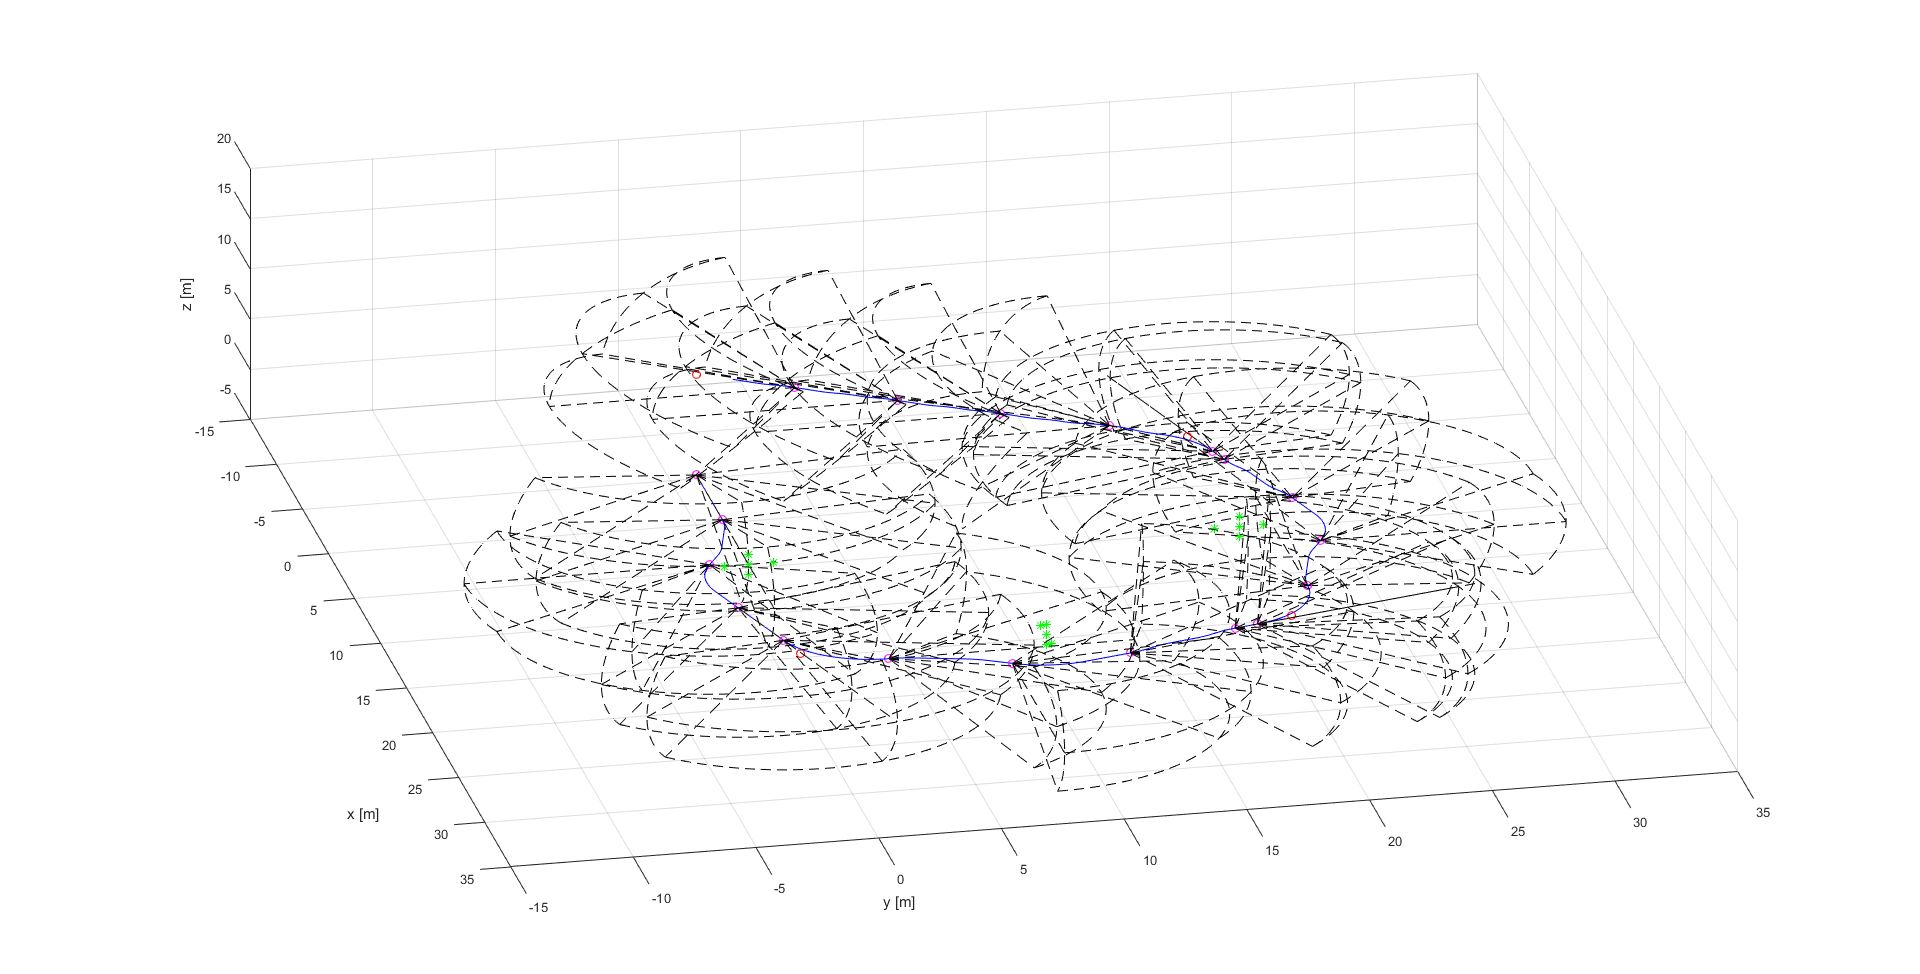
\includegraphics[width=\linewidth]{\FIGDIR/42_Known_world_during_flight.png}
    \caption{Known world during flight in virtual playground.}
    \label{fig:knownWorldDuringFlight}
\end{figure}

\noindent For testing purposes simple cost function $J^*(x(t_i),\mathscr{MA}(t_i))$ is defined for pre-calculated maximal reach set $\mathscr{R}(t_0,t_1,x_0)$ given by def. \ref{def:NumericReachSet3D}. Cost function $J^*$ (\ref{eq:simpleCostFunctionReachSetTest}) is calculated for discrete avoidance time $t_i$ as Euclidean position difference for vehicle position $[x_v,y_v,z_v]$ with penalisation coefficient $c_p(m_k)$ (\ref{eq:penalisationCoeficientSimple}).
\begin{equation}\label{eq:simpleCostFunctionReachSetTest}
    J^*(x(t_i),\mathscr{MA}(t_i) = \sum_{k=1}^i \left(\sqrt{ 
    \begin{aligned}
    &\left(x_v(t_k)-x_v(t_{k-1})\right)^2\\
    +&\left(y_v(t_k)-y_v(t_{k-1})\right)^2\\
    +&\left(z_v(t_k)+z_v(t_{k-1})\right)^2 
    \end{aligned}}\right)c_p(m_k) 
\end{equation}
Purpose of penalisation coefficient $c_p(m_k)$ (\ref{eq:penalisationCoeficientSimple}) is to prefer movements in order: straight($\circledcirc$), right($\Rightarrow$), left($\Leftarrow$), up($\Uparrow$) and down($\Downarrow$). For each trajectory $\mathscr{T}(x_0,B)$ passing trough goal cell $c_{i,j,k}$ cost $J^*$ is assigned, therefore goal determination algorithm (alg. \ref{alg:goalSelectionExample}.) can select best avoidance trajectory $\mathscr{T}(x_0,B)$ in avoidance framework inner cycle (alg. \ref{alg:avoidanceFramework}).
\begin{equation}\label{eq:penalisationCoeficientSimple}
    c_p(m_k)=
    \begin{cases}
        1 :&\text{if} m_k =\circledcirc \\
        1.5 :&\text{if} m_k = \Leftarrow\text{ or }m_k = \Rightarrow\\
        2 :\text{if}& m_k = \Uparrow\text{ or }m_k = \Downarrow
    \end{cases}
\end{equation}
Let say that testing vehicle is occupying in unit-ball $\mathscr{B}$ with diameter $0.30$ m, therefore minimal safety margin is $s_m=0.3m$. Turning radius of vehicle is $2$ meters. If potentional field method is used \cite{koren1991potential}. Minimal safety margin $s_m$ of  $2.6$ meters will be used. Presented obstacle avoidance framework can potentially reduce safety margin $s_m$ to diameter of vehicle unit ball $\mathscr{B}$ and predicted trajectory error $e_p$. Because prediction error $e_p$ have been measured in worst case scenario as $0.3$ meters, therefore safety margin $s_m$ is set as $0.6$ meters. 

Standard LiDAR sensor can scan up to $200$ meters in front of the vehicle. Let us assume very bad weather conditions. According to case study \cite{ramasamy2016lidar} worst possible visibility range in fog with heavy rain is $10$ meters. Using these parameters testing visibility grid is defined as equation \ref{eq:FOVsim3D}.
\begin{equation}\label{eq:FOVsim3D}
    \mathscr{G}_{3D}(d_s=0m,d_e=10m,\theta_s = \frac{\pi}{3},\theta_e =-\frac{\pi}{3},\varphi_s =\frac{pi}{6},\varphi_e=-\frac{pi}{6}).     
\end{equation}


\noindent Movement automaton $\mathscr{MA}$ buffer $B_{\mathscr{MA}}$ is filled with 1 to 10 movements based on actual avoidance grid $\mathscr{A}(t_i)$. at time of avoidance execution $t_i$. Obstacle avoidance algorithm is executed every time when vehicle moves half of visibility grid (every $\sim$5 s). When avoidance algorithm finishes ($\sim$ 0.5 s) movement automaton buffer $B_{\mathscr{MA}}$ is flushed and previously planned movements are replaced with new ones.

Two separate cases are considered to verify aspects of avoidance framework given by alg. \ref{alg:avoidanceFramework}.:
\begin{enumerate}
    \item \textit{Simple obstacle avoidance} - vehicle flies between two waypoints and encounters obstacles, this case shows decision making of obstacle avoidance framework.
    \item \textit{Mission plan execution} - vehicle executes mission plan defined in section \ref{ch:3DPlaygroundDefinition}, this case is to show complex mission execution, and discuss overall framework performance.
\end{enumerate}

\subsection{Simple obstacle avoidance}
\noindent Avoidance decision time $t_d$ is important parameter, because it is definef visibility grid $\mathscr{G}_{3D}$ overlaps in known world $\mathscr{F}$. Every decision time $t_d$ obstacle avoidance framework (alg. \ref{alg:avoidanceFramework}) is executed. For purpose of this simulation Movement automaton structure (def. \ref{def:movementAutomaton}.) is extended for:
\begin{enumerate}
    \item \text{Executed buffer} $B_E\in M^i$ - purpose is to store executed movements in decision time $t_0+kt_{d+1},k\in\N^+$, movements are stored after next decision frame $\mathscr{D}(t_d+1)$is invoked.
    \item \text{Planned buffer} $B_P\in M^i$ - purpose is to store planned movements in decision time $t_0+kt_{d},k\in\N^+$., movements are stored when actual decision frame is invoked $\mathscr{D}(t_d)$.
\end{enumerate}
Decision frame $\mathscr{D}(t_d)$  is deployed every decision time $t_d$. Six decision frames were deployed during this simulation. Main purpose is to show how decision frame impacts planned and flew trajectory.


For simple obstacle avoidance mission plan is defined by waypoint set $\mathscr{WP}$ (\ref{eq:simpleObstacleMissionPG1}) and obstacle set $\mathscr{O}$ (\ref{eq:simpleObstacleMissionPG2}). There is two waypoints $\mathscr{WP_S}$ and $\mathscr{WP}_E$ with mutual distance $30m$.
\begin{equation}\label{eq:simpleObstacleMissionPG1}
    \mathscr{WP}=\left\{\mathscr{WP}_S,\mathscr{WP}_E\right\} = \left\{[0,0,0],[30,0,0]\right\}
\end{equation}
Two obstacle sets $\mathscr{O}_1$ and $\mathscr{O}_2$ are put between waypoints $\mathscr{WP_S}$ and $\mathscr{WP}_E$ (\ref{eq:simpleObstacleMissionPG1}). Its assured that vehicle without avoidance system will crash into obstacle set $\mathscr{O}$.
\begin{equation}\label{eq:simpleObstacleMissionPG2}
    \begin{aligned}
    \mathscr{O}   &= \left\{\mathscr{O}_1,\mathscr{O2}\right\}\\
    \mathscr{O}_1 &= \left\{[10,0,0],[10,1,0)[10,-1,0],[10,0,1],[10,0,-1]\right\}\\
    \mathscr{O}_2 &= \left\{[10,0,0],[10,1,0)[10,-1,0],[10,0,1],[10,0,-1]\right\}
    \end{aligned}
\end{equation}

\noindent Decision frame is invoked $t_d=5s$, mission given by wapypoints $\mathscr{WP}$ and  obstacles $\mathscr{O}$ had six decisions frames defined at decision time $t_d\in T_d = \left\{0, 5, 10, 15, 20, 25\right\}$. Decisions made in decision time set $T_d$ are discussed in following text

\begin{figure}[H]
    \centering
    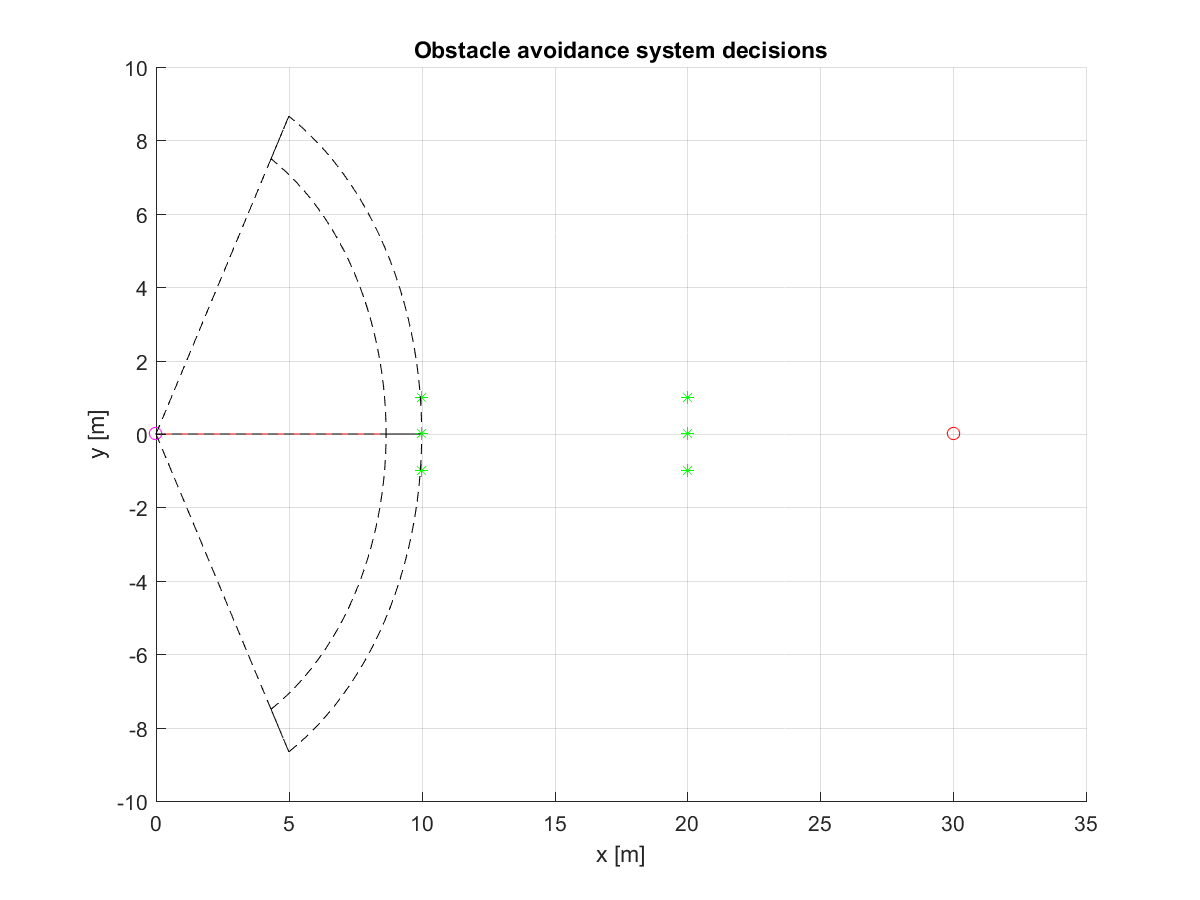
\includegraphics[width=0.7\linewidth]{\FIGDIR/64_AvoidanceFrame-01.png}
    \caption{Decision frame $\mathscr{D}(0)$.}
    \label{fig:decisionFrameSimple0}
\end{figure}
\noindent Decision $\mathscr{D}(0)$ is portrayed in figure \ref{fig:decisionFrameSimple0}. Vehicle is at initial position $x_0$ and visibility grid $\mathscr{G}_3D$ does not registered any approaching obstacle, therefore avoidance grid $\mathscr{A}(0)$ is identical to maximal avoidance grid. Goal cell $c_{i,j,k}$ is selected as closest cell to $\mathscr{WP}_E$. Planned movement buffer $B_P$ is filled with movement buffer from trajectory $\mathscr{T}(x_0,B)$. Five straight movement $\circledcirc(5)$ are executed as results. Without executing avoidance at decision time $t_d=5$ vehicle will surely crash to obstacle set $\mathscr{O}_1$.
Planned buffer $B_P$ for decision frame $\mathscr{D}(0)$ have following values $B_P$ = \textit{[$\mathscr{D}(0)$ $\circledcirc$(10)]}.
Executed buffer $B_E$ for decision frame $\mathscr{D}(0)$ have following values $B_P$ = \textit{[$\circledcirc$(5)]}.
\begin{figure}[H]
    \centering
    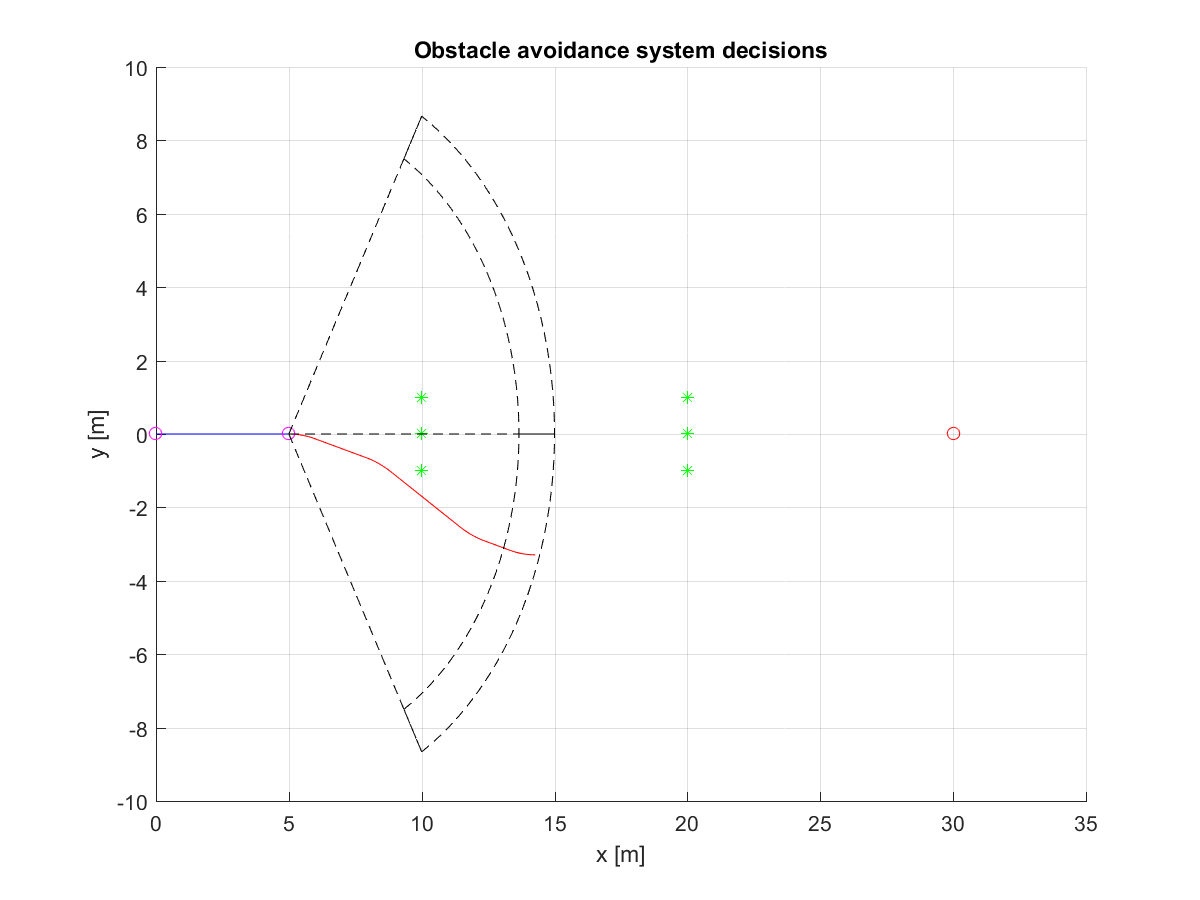
\includegraphics[width=0.7\linewidth]{\FIGDIR/65_AvoidanceFrame-02.png}
    \caption{Decision frame $\mathscr{D}(5)$.}
    \label{fig:decisionFrameSimple5}
\end{figure}
\newpage
\noindent Decision $\mathscr{D}(5)$ is portrayed in figure \ref{fig:decisionFrameSimple5}. Vehicle executed five of movements $m_i$ planned in decision frame $\mathscr{D}(0)$. Visibility grid $\mathscr{G}_{3D}$ is filled with obstacle set $\mathscr{O_1}$. Avoidance grid $\mathscr{A}(5)$ asses space inf front of the obstacle set $\mathscr{O}_1$ as \textit{'Uncertain'}, therefore any trajectory $\mathscr{T}(x_5,B)$ belonging to reduced reach set $\mathscr{R}(t_5,t_{10},x_{5})$ does not return to original course after passing an obstacle. Avoidance trajectory $\mathscr{A}(x_5,B)$ with lowest cost $J^*$ selected in goal cell $c_{i,j,k}$ closest to waypoint $\mathscr{WP}_E$. Avoidance priority is \text{straight, right, left, up and down}, because \text{straight} trajectory is not available \textit{right} avoidance trajectory is selected. Planed trajectory $\mathscr{T}(x_5,B_P)$ is deviating from original course, but is deemed as safe trajectory.
Planned buffer $B_P$ for decision frame $\mathscr{D}(5)$ have following values $B_P$ = \textit{[ $\Rightarrow$(1), $\circledcirc$(2), $\Rightarrow$(1), $\circledcirc$(3), $\Leftarrow$(1), $\Downarrow$(1), $\Leftarrow$(1)]}.
Executed buffer $B_E$ for decision frame $\mathscr{D}(5)$ have following values $B_P$ = \textit{[$\Rightarrow$(1), $\circledcirc$(2), $\Rightarrow$(1), $\circledcirc$(1)]}.     
\begin{figure}[H]
    \centering
    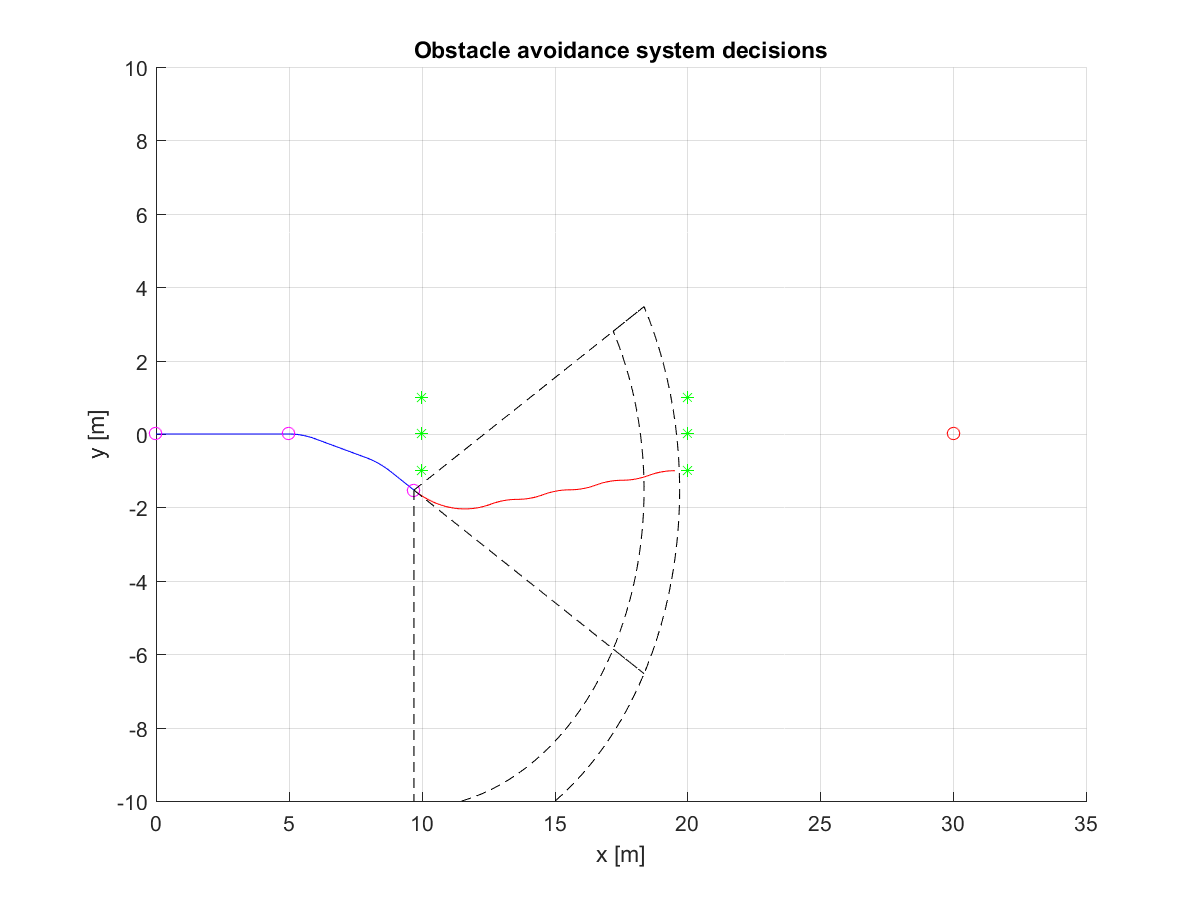
\includegraphics[width=0.7\linewidth]{\FIGDIR/66_AvoidanceFrame-03.png}
    \caption{Decision frame $\mathscr{D}(10)$.}
    \label{fig:decisionFrameSimple10}
\end{figure}
\noindent Decision $\mathscr{D}(10)$ is portrayed in figure \ref{fig:decisionFrameSimple10}. Vehicle executed five of movements $m_i$ planned in decision frame $\mathscr{D}(5)$. Visibility grid $\mathscr{G}_{3D}$. does not register obstacle set $\mathscr{O}_2$, because its behind border of vision. Avoidance grid $\mathscr{A}(t_{10})$ is loaded with maximal reach set $\mathscr{R}(t_{10},t_{15},x_{10})$. Goal cell $c_{i,j,k}$ with cheapest trajectory $\mathscr{T}(x_{10},B_P)$ is selected. At this state vehicle is planning to return to original trajectory between waypoints $\mathscr{WP}_S$ and $\mathscr{WP}_E$. If planned buffer $B_P$ was fulle executed at this state $x_{10}$, it will lead to crash at obstacle set $\mathscr{O}_2$.
Planned buffer $B_P$ for decision frame $\mathscr{D}(10)$ have following values $B_P$ = \textit{ [$\Leftarrow$(3), $\Rightarrow$(1), $\Leftarrow$(1), $\Rightarrow$(1), $\Leftarrow$(1), $\Rightarrow$(1), $\Leftarrow$(1), $\Rightarrow$(1)]}.
Executed buffer $B_E$ for decision frame $\mathscr{D}(10)$ have following values $B_P$ = \textit{[$\Leftarrow$(3), $\Rightarrow$(1), $\Leftarrow$(1]}.
\begin{figure}[H]
    \centering
    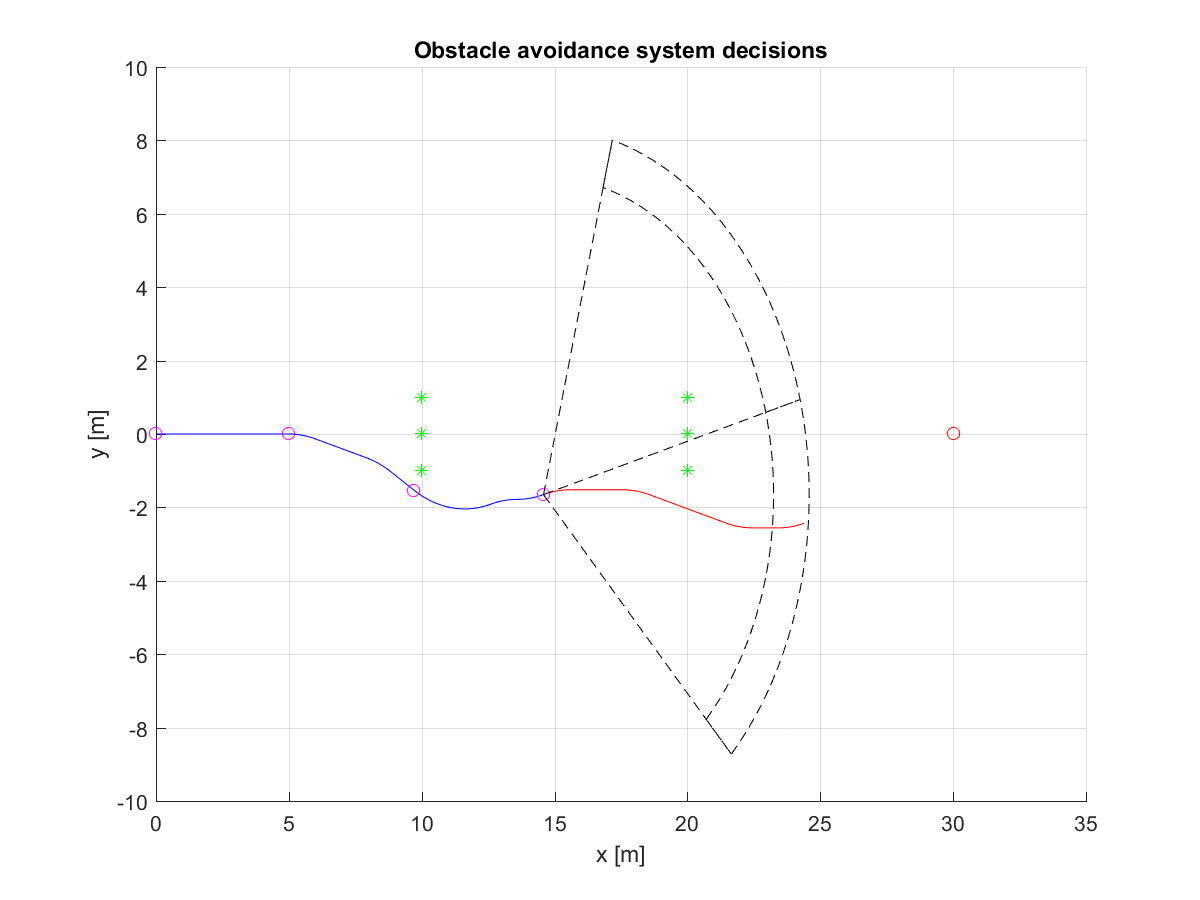
\includegraphics[width=0.7\linewidth]{\FIGDIR/67_AvoidanceFrame-04.png}
    \caption{Decision frame $\mathscr{D}(15)$.}
    \label{fig:decisionFrameSimple15}
\end{figure}
\noindent Decision $\mathscr{D}(15)$ is portrayed in figure \ref{fig:decisionFrameSimple15}. Vehicle executed five of movements $m_i$ planned in decision frame $\mathscr{D}(10)$. Visibility grid $\mathscr{G}_{3D}$ has detected obstacle set $\mathscr{O}_2$. Avoidance grid $\mathscr{A}(t_{15})$ is initialized and pruned, reduced reach set $\mathscr{R}(t_{15},t_{20},x_{15})$ is obtained. Goal cell $c_{i,j,k}$ closest to waypoint $\mathscr{WP}_E$ is selected. Trajectory $\mathscr{T}(x_{15},B_P)$ with lowest cost function $J*$ is selected as avoidance trajectory. Avoidance maneuver is avoiding detected obstacle set $\mathscr{O}_2$ from right side, due the avoidance maneuvers priority. 
Planned buffer $B_P$ for decision frame $\mathscr{D}(15)$ have following values $B_P$ = \textit{
[$\Rightarrow$(1), $\circledcirc$(2), $\Rightarrow$(1), $\circledcirc$(3), $\Leftarrow$(1), $\Downarrow$(1), $\Leftarrow$(1)]}.
Executed buffer $B_E$ for decision frame $\mathscr{D}(10)$ have following values $B_P$ = \textit{[$\Rightarrow$(1), $\circledcirc$(2), $\Rightarrow$(1), $\circledcirc$(1)]}.
\begin{figure}[H]
    \centering
    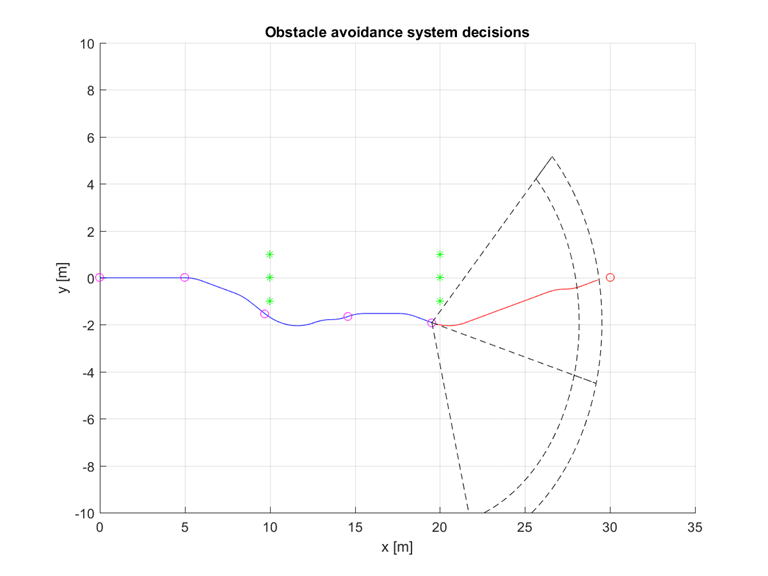
\includegraphics[width=0.7\linewidth]{\FIGDIR/68_AvoidanceFrame-05.png}
    \caption{Decision frame $\mathscr{D}(20)$.}
    \label{fig:decisionFrameSimple20}
\end{figure}
\noindent Decision $\mathscr{D}(20)$ is portrayed in figure \ref{fig:decisionFrameSimple20}. Vehicle executed five of movements $m_i$ planned in decision frame $\mathscr{D}(15)$. Visibility grid $\mathscr{G}_{3D}$ does not contain any obstacle, therefore shortest trajectory $\mathscr{T}(x_20,B_P)$ to $\mathscr{WP}_E$ is selected as avoidance trajectory. This decision is standard after avoidance decision and vehicle will return to original trajectory between $\mathscr{WP}_S$ and $\mathscr{WP}_E$.
Planned buffer $B_P$ for decision frame $\mathscr{D}(20)$ have following values $B_P$ = \textit{[$\Leftarrow$(2), $\circledcirc$(5), $\Rightarrow$(1), $\Leftarrow$(1), $\circledcirc$(1)]}.
Executed buffer $B_E$ for decision frame $\mathscr{D}(20)$ have following values $B_P$ =\textit{[$\Leftarrow$(2), $\circledcirc$(3)]}.
\begin{figure}[H]
    \centering
    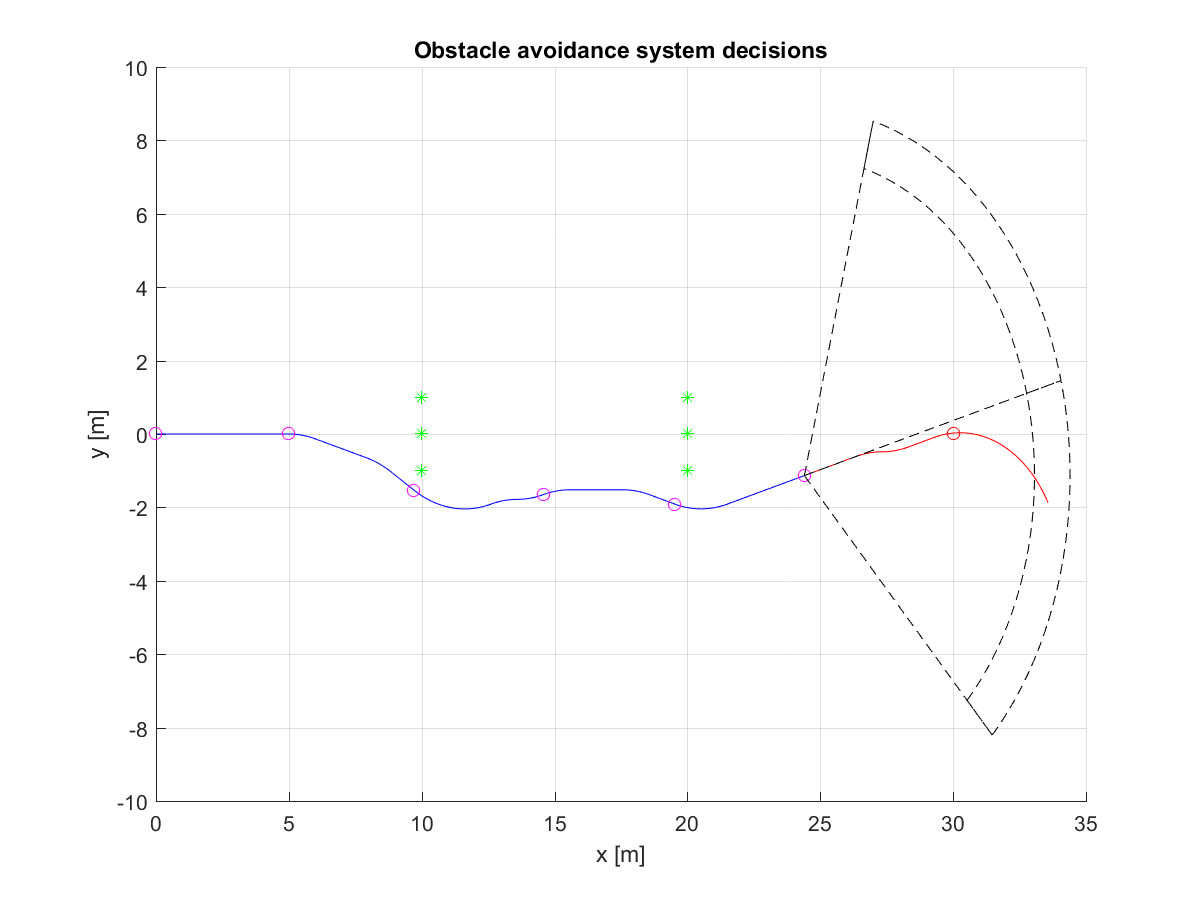
\includegraphics[width=0.7\linewidth]{\FIGDIR/69_AvoidanceFrame-06.png}
    \caption{Decision frame $\mathscr{D}(25)$.}
    \label{fig:decisionFrameSimple25}
\end{figure}
\noindent Decision $\mathscr{D}(25)$ is portrayed in figure \ref{fig:decisionFrameSimple25}. Waypoint $\mathscr{WP}_E$ will be reached after execution of first five movement $m_i$. Other half of planned movements is unused.
Planned buffer $B_P$ for decision frame $\mathscr{D}(25)$ have following values $B_P$ =  \textit{[$\circledcirc$(2), $\Rightarrow$(1), $\Leftarrow$(1), $\circledcirc$(1) $\Rightarrow$(5)]}.
Executed buffer $B_E$ for decision frame $\mathscr{D}(25)$ have following values $B_P$ = \textit{[$\circledcirc$(2), $\Rightarrow$(1), $\Leftarrow$(1), $\circledcirc$(1)]}.
\begin{figure}[H]
    \centering
    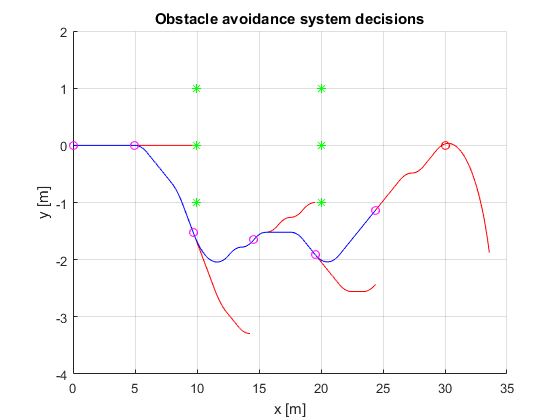
\includegraphics[width=0.7\linewidth]{\FIGDIR/70_PathPlanning_vs_Execution.png}
    \caption{Planned movements (red) vs. Executed movements (blue).}
    \label{fig:planVSExecutionSimple}
\end{figure}
\noindent Aggregated view of all planned movements $\cup B_P(i)$ (red) and all executed movements $\cup B_E(i)$ (blue) for decision frames $\mathscr{D}(t_d);t_d=\{0,5,10,15,25\}$ is portrayed in figure \ref{fig:planVSExecutionSimple}. Two collision situations were inverted in frames $\mathscr{D}(10)$ to obstacle set $\mathscr{O}_1$ and $\mathscr{D}(20)$ to obstacle set $\mathscr{O}_2$.
\begin{figure}[H]
    \centering
    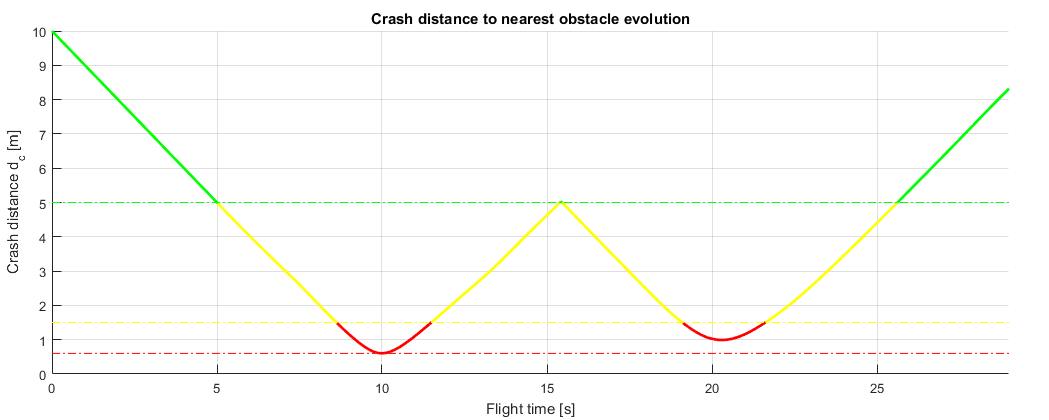
\includegraphics[width=0.8\linewidth]{\FIGDIR/61_Crash_distance_to_nearest_obstacle_evolution_known_world.png}
    \caption{Vehicle crash distance $d_c$ evolution during flight}
    \label{fig:vehicleCrashDistanceEvolutionDecisions}
\end{figure}
\noindent Crash distance $d_c$ evolution is portrayed in figure \ref{fig:vehicleCrashDistanceEvolutionDecisions}. Minimal crash distance $d_c$ never crossed safety margin $s_m$ therefore safety condition $min(d_c)\ge s_m$ is considered as satsfied. 

\subsection{Mission plan execution}
\noindent Vehicle executes mission plan defined in section \ref{ch:3DPlaygroundDefinition}. This simulation considers only notable detection frames $\mathscr{D}(t_d)$ at time of decision $t_d$. This cased shows what happens during complex mission execution.

Movement between waypoints are portrayed in figures \ref{fig:43firstwaypointMovement}, \ref{fig:45secondwaypointMovement}, \ref{fig:47thirdwaypointMovement}, \ref{fig:fourthObstacleGrid}. \textit{Red circles} represents waypoints $\mathscr{WP}$, \textit{magenta circles} represents avoidance decision points $\mathscr{D}(t_d)$, \text{blue line} represents vehicle trajectory in $\R^3$, \textit{black dashed line} represents visibility gird $\mathscr{G}_{3D}$ in time of obstacle avoidance $t_i$, \textit{green stars} represents detected obstacle points $o_i\in\mathscr{O}\subset\mathscr{G}_{3D}$.

Obstacle avoidance in given visibility grid $\mathscr{G}_{3D}$ during escape calculation are portrayed in figures \ref{fig:44ObstacleAvoidance}, \ref{fig:46ObstacleAvoidance}, \ref{fig:48ObstacleAvoidance}. \textit{Cyan dashed line} represents boundary of visibility cells $c_{i,j,k}$ in avoidance grid $\mathscr{A}(t_d)$. Each cell state is represented by point at their center, for reachable cells \textit{green cross} is used, for unreachable cells \textit{black cross} is used, for obstacle cells \textit{red circle is used}, for uncertain cells \textit{magenta circle} is used. avoidance trajectory $\mathscr{T}(x_{t_d},B)$ from reduced reach set $\mathscr{R}(t_d,t_{d+5},x_{t_d})$ is displayed as \textit{red line}.
\begin{figure}[H]
    \begin{subfigure}{0.5\textwidth}
    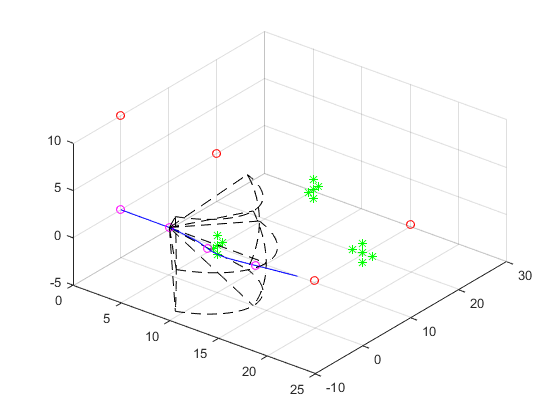
\includegraphics[width=0.9\linewidth]{\FIGDIR/43_First_waypoint_movement.png} 
    \caption{Movement to waypoint.}
    \label{fig:43firstwaypointMovement}
    \end{subfigure}
    \begin{subfigure}{0.5\textwidth}
    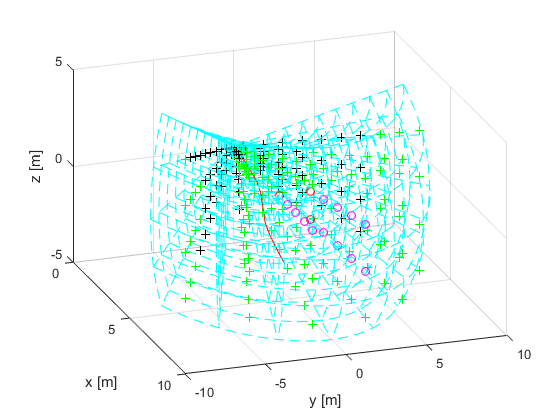
\includegraphics[width=0.9\linewidth]{\FIGDIR/44_First_osbtacle_avoidance.png}
    \caption{Avoidance grid $\mathscr{A}(t_5)$}
    \label{fig:44ObstacleAvoidance}
    \end{subfigure}
\caption{Obstacle avoidance at $\mathscr{WP}_1=[20,0,0]^T$, with best avoidance maneuver in reachable set.}
\label{fig:firstObstacleGrid}
\end{figure}
\noindent Vehicle encounters first obstacle set $\mathscr{O}_1$ at decision time $t_d=5s$. Avoidance grid $\mathscr{A}(t_5)$is initialized and filled with obstacles, reduced reach set $\mathscr{R}(t_5,t_{10},x_{5})$ is obtained. Right avoidance is executed and vehicle continues to move to goal waypoint $\mathscr{WP}_1$.
Executed movements during flight from $\mathscr{WP}_S$ to $\mathscr{WP}_1$ have follow values: $B_{\mathscr{MA}}$ = \textit{[$\circledcirc$(5), right(1), $\circledcirc$(2), $\Rightarrow$(1), $\circledcirc$(1), $\Leftarrow$(3), $\circledcirc$(6)]}
\begin{figure}[H]
    \begin{subfigure}{0.5\textwidth}
    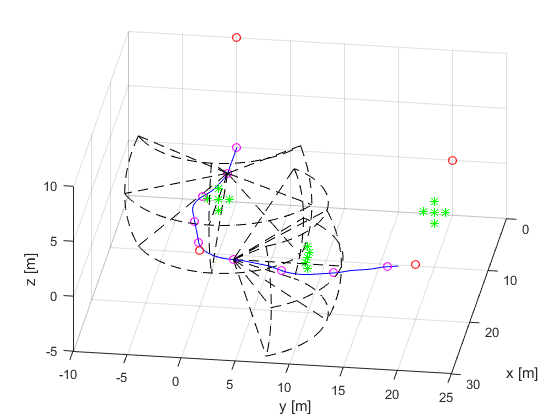
\includegraphics[width=0.9\linewidth]{\FIGDIR/45_Second_waypoint_movement.png} 
    \caption{Movement to waypoint.}
    \label{fig:45secondwaypointMovement}
    \end{subfigure}
    \begin{subfigure}{0.5\textwidth}
    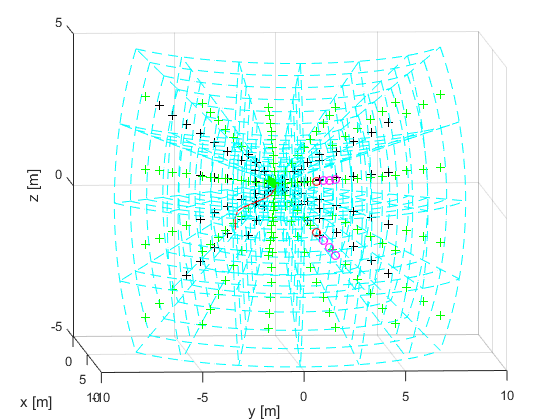
\includegraphics[width=0.9\linewidth]{\FIGDIR/46_Second_obstacle_avoidance.png}
    \caption{Avoidance grid $\mathscr{A}(t_{25}$}
    \label{fig:46ObstacleAvoidance}
    \end{subfigure}
\caption{Obstacle avoidance at $\mathscr{WP}_2=[20,20,0]^T$. with best avoidance maneuver in reachable set.}
\label{fig:secondObstacleGrid}
\end{figure}
\newpage
\noindent Vehicle reaches waypoint $\mathscr{WP}_1$ and sets waypoint $\mathscr{WP}_2$ as new goal waypoint. Vehicle executes sharp left turn. Obstacle set $\mathscr{O}_2$ is detected at time of decision $t_d=25s$. Similar maneuvers are executed as in case of obstalce set $\mathscr{O}_1$.
Executed movements buffer during flight from $\mathscr{WP}_1$ to $\mathscr{WP}_2$ have follow values: $B_{\mathscr{MA}}$ = \textit{[$\Leftarrow$(5), right(1), $\circledcirc$(2), right(1), $\circledcirc$(1), $\Leftarrow$(3), $\circledcirc$(1), $\Leftarrow$(1), right(1), $\circledcirc$(1), $\Leftarrow$(1), right(1), $\circledcirc$(1)]}.
\begin{figure}[H]
    \begin{subfigure}{0.5\textwidth}
    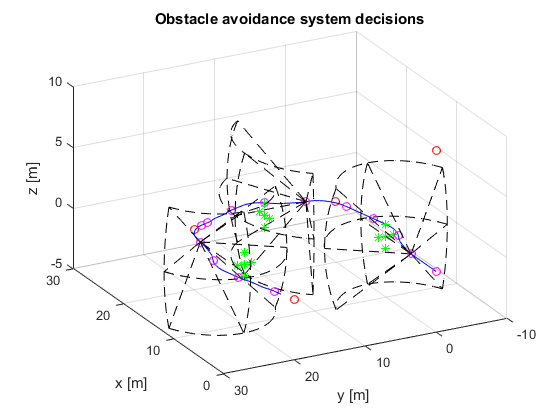
\includegraphics[width=0.9\linewidth]{\FIGDIR/47_Third_waypoint_movement.png} 
    \caption{Movement to waypoint.}
    \label{fig:47thirdwaypointMovement}
    \end{subfigure}
    \begin{subfigure}{0.5\textwidth}
    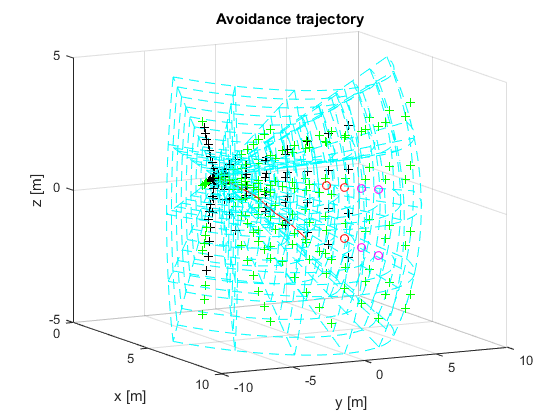
\includegraphics[width=0.9\linewidth]{\FIGDIR/48_Third_obstacle_avoidance.png}
    \caption{Avoidance grid $\mathscr{A}(t_{50})$}
    \label{fig:48ObstacleAvoidance}
    \end{subfigure}
\caption{Obstacle avoidance at $\mathscr{WP}_3=[0,20,0]^T$. with best avoidance maneuver in reachable set.}
\label{fig:thirdObstacleGrid}
\end{figure}
\noindent Vehicle reaches waypoint $\mathscr{WP}_2$ and sets waypoint $\mathscr{WP}_3$ as new goal waypoint. Vehicle executes sharp left turn. Obstacle set $\mathscr{O}_3$ is detected at time of decision $t_d=50s$. Similar maneuvers are executed as in case of obstalce set $\mathscr{O}_2$.
Executed movements during flight from $\mathscr{WP}_2$ to $\mathscr{WP}_3$ have follow values: $B_{\mathscr{MA}}$ = \textit{[$\Leftarrow$(5), right(1), $\circledcirc$(2), right(1), $\circledcirc$(1), $\Leftarrow$(3), $\circledcirc$(1), $\Leftarrow$(1), right(1), $\circledcirc$(1), $\Leftarrow$(1), right(1), $\circledcirc$(1)]}.
\begin{figure}[H]
    \centering
    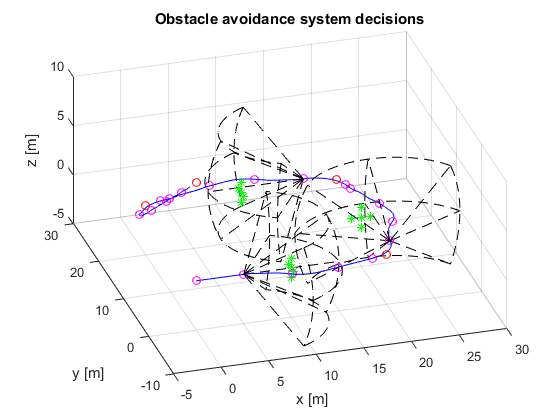
\includegraphics[width=0.6\linewidth]{\FIGDIR/49_Fourth_waypoint_movement.png}
    \caption{Optimal minimal cost flight to $\mathscr{WP}_E=[0,0,10]^T$, no avoidance have been executed.}
    \label{fig:fourthObstacleGrid}
\end{figure}
\newpage
\noindent Vehicle reaches waypoint $\mathscr{WP}_3$ and sets waypoint $\mathscr{WP}_E$ as new goal waypoint. Vehicle executes sharp left turn with increasing altitude to reach final waypoint $\mathscr{WP}_E$. 
Movement automaton buffer during flight from $\mathscr{WP}_3$ to $\mathscr{WP}_E$ have follow values: $B_{\mathscr{MA}}$ = \textit{[$\Leftarrow$(3), $\Uparrow$(1), $\Leftarrow$(2), $\Uparrow$(1), $\Leftarrow$(1), right(1), $\circledcirc$(1) ,$\Leftarrow$(1), right(1), $\Leftarrow$(1), right(1), $\circledcirc$(1), $\Leftarrow$(1), right(1), $\Leftarrow$(1), right(1), $\circledcirc$(1), $\Leftarrow$(1), right(1), $\circledcirc$(1)]}.
Simulation stops when final waypoint $\mathscr{WP}_E$ is reached.

\begin{figure}[H]
    \centering
    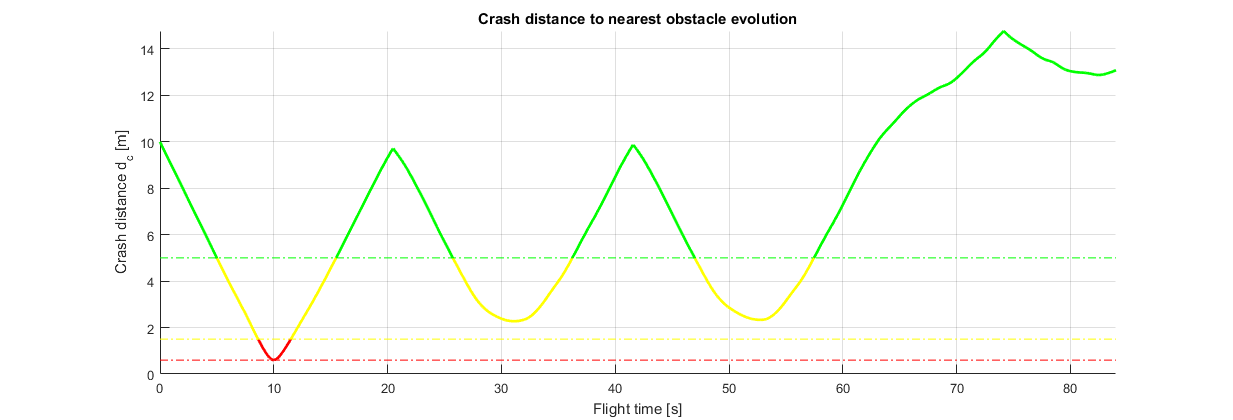
\includegraphics[width=0.95\linewidth]{\FIGDIR/59_Crash_distance_to_nearest_obstacle_evolution.png}
    \caption{Vehicle crash distance $d_c$ evolution during flight}
    \label{fig:vehicleCrashDistanceEvolution}
\end{figure}
\noindent Vehicle crash distance $d_c$ evolution during flight simulation have been measured to closest known obstacle $o_i\in\mathscr{O}$ in known world $\mathscr{F}$.  Figure \ref{fig:vehicleCrashDistanceEvolution}. shows crash distance evolution. Distance have been divined into following levels:
\begin{enumerate}
    \item \textit{Safe distance (green)} - distance where crash is avoidable, in this case $distance \ge 5 m$, this distance is threshold for conservative methods. 
    \item \textit{Cautious distance (yellow)} - distance where crash is avoidable with additional effort using special maneuver, in this case $1.5m \ge distance < 5m$, this distance is best performance for methods with obstacle classification.
    \item \textit{Dangerous distance (red)} - distance where crash is invertible in case of noncolinear obstacle heading, in this case $0.6m \ge distance < 1.5m$, this distance can be only performed by presented obstacle avoidance algorithm.
\end{enumerate}
\noindent During simulation only closest distance to obstacle of 0.7 meter have been reached. This proves that presented avoidance algorithm keeps given safety margin $s_m=0.6 m$ also in practical implementation. The theoretical obstacle distance is best in state of art of theoretical avoidance systems.

Prediction quality is very important factor in predictive control, therefore quantitative measurement for prediction of this system have been introduced (\ref{eq:movementAutomatonPredictionError2}). Movement automaton prediction error $e_p$ is based on mean square prediction error (MSE).
\begin{equation}\label{eq:movementAutomatonPredictionError2}
    e_p=\sqrt{\sum_{t_i=t_0+i}^{i\in\{1,\dots,n\}} \left (\hat{x}(t_i)-x(t_i)\right)^2}    
\end{equation}

\noindent Movement automaton prediction error compares predicted state $\hat{x}$ and real system state $x$ for each movement execution time $t_i$. Movement execution time in this case was $s_1$ so time $t_i$ was defined as $t_i=t_0+i, i\in\{1,\dots,n\}$, where n is total count of executed movements. Movement automaton prediction error $e_p$ was in this case $e_p\approx 0$.
\begin{figure}[H]
    \centering
    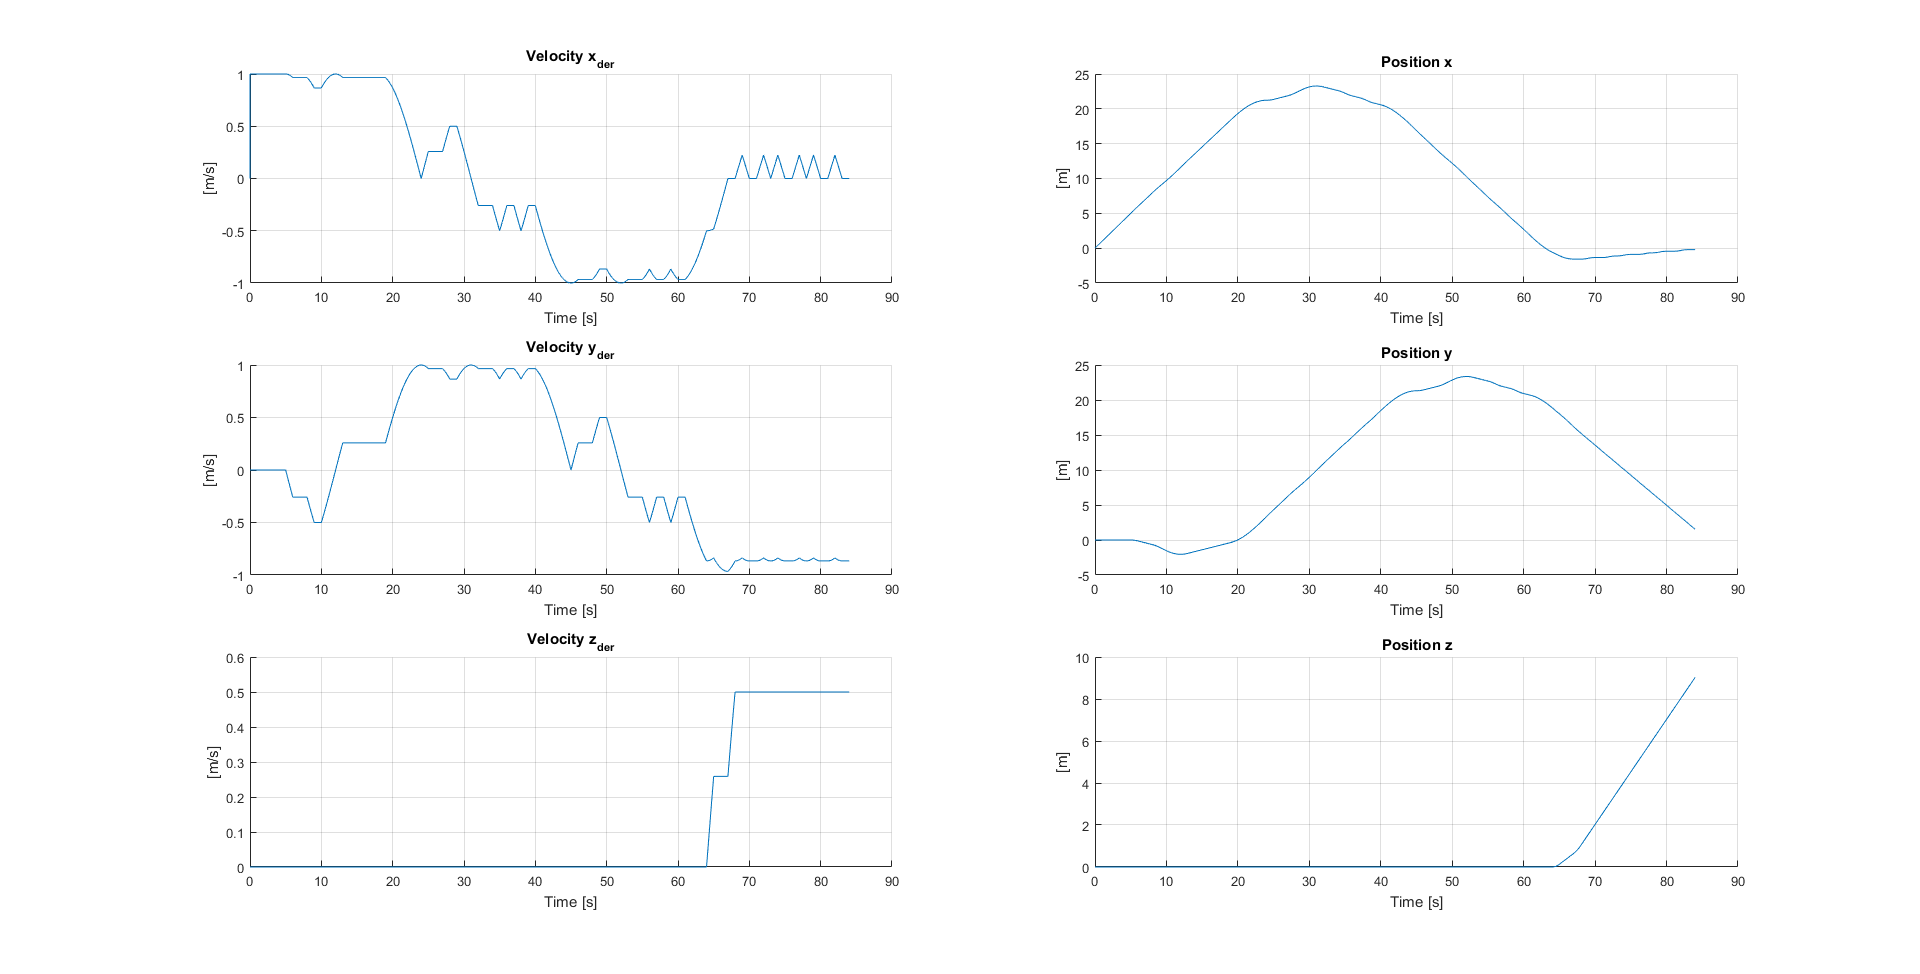
\includegraphics[width=\linewidth]{\FIGDIR/50_Vehicle_position.png}
    \caption{Vehicle position $x,y,z$ and their derivations $\dot{x},\dot{y},\dot{z}$ evolution during flight.}
    \label{fig:vehicleStateGrid1}
\end{figure}
\noindent Vehicle position $x,y,z$ and their derivations $\dot{x},\dot{y},\dot{z}$ and their evolution during flight is portrayed in figure \ref{fig:vehicleStateGrid1}. Brown color is used for predicted model state and blue color is used for real model parameter evolution. Both models are equal, supported by movement automaton prediction error $e_p\approx 0$.
\begin{figure}[H]
    \centering
    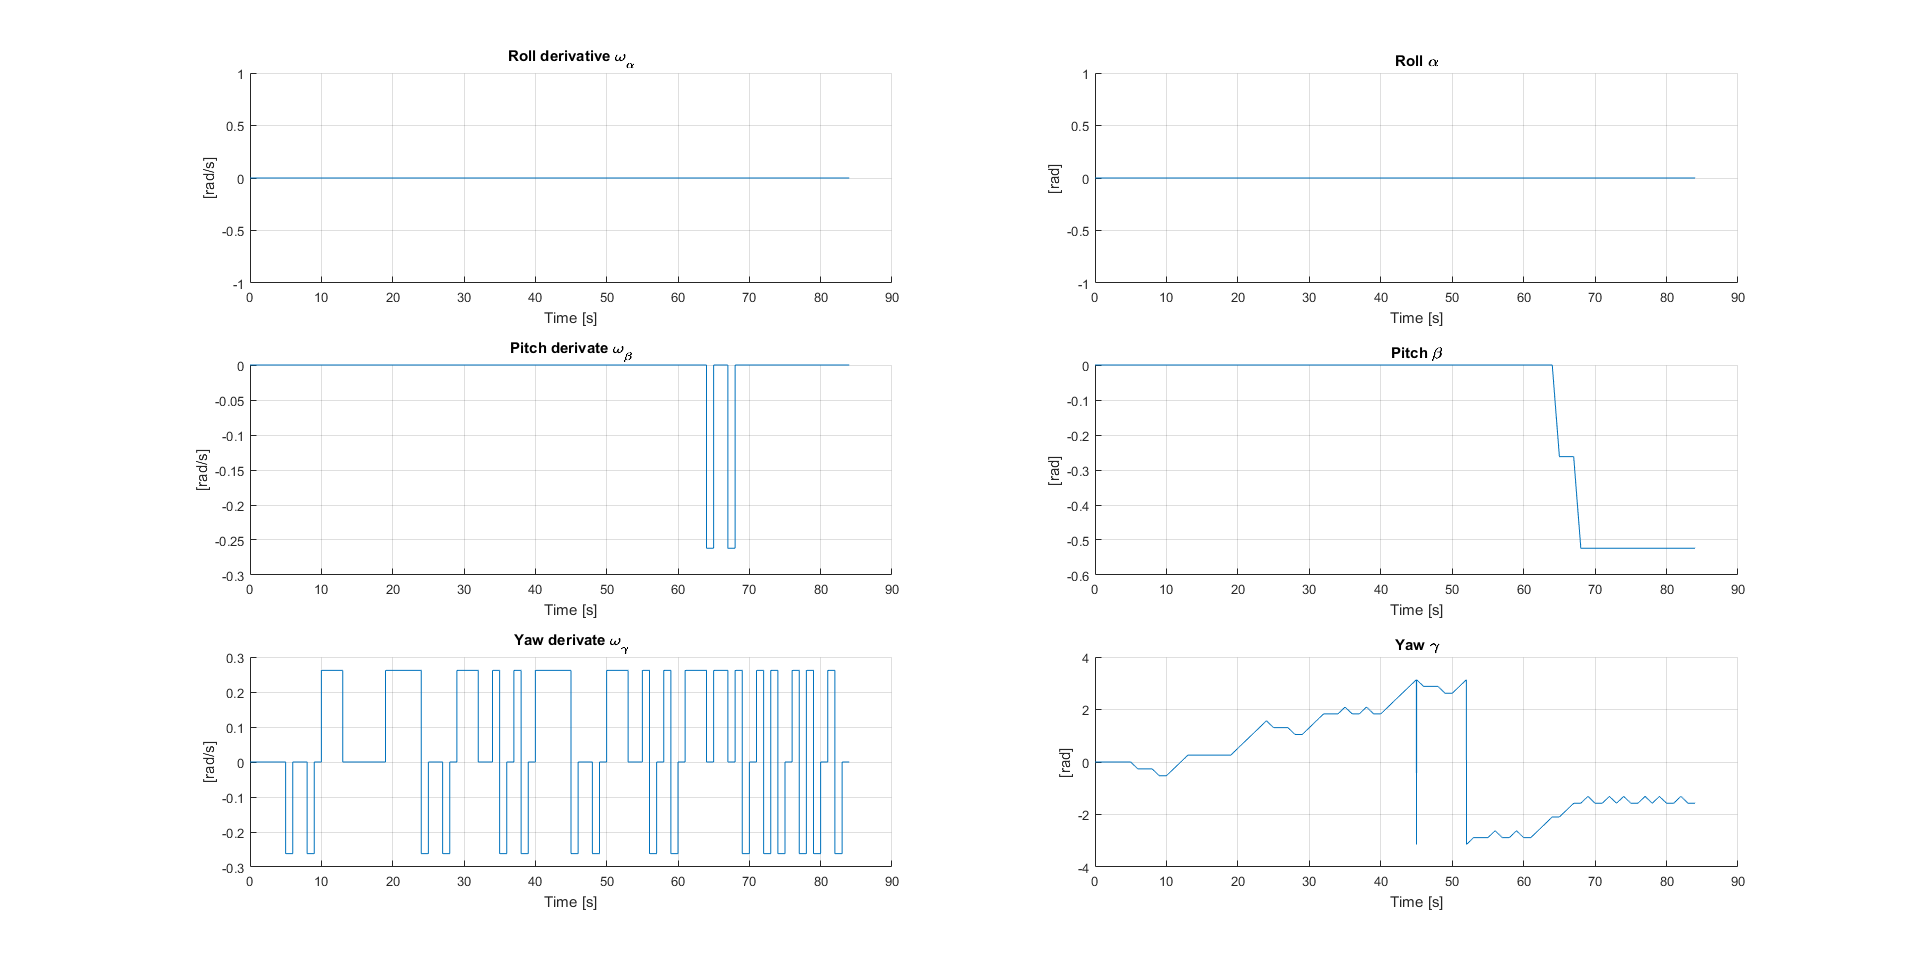
\includegraphics[width=\linewidth]{\FIGDIR/51_Vehicle_angles.png}
    \caption{Vehicle positional angles $\alpha,\beta,\gamma$ and their angular velocities $\omega_\alpha,\omega_\beta,\omega_\gamma$ evolution during flight}
    \label{fig:vehicleStateGrid2}
\end{figure}
\noindent Similar to previous comparison (fig. \ref{fig:vehicleStateGrid1}.) Comparison for vehicle positional angles $\alpha,\beta,\gamma$ and their angular velocities $\omega_\alpha,\omega_\beta,\omega_\gamma$ evolution during flight holds previous assumption (fig. \ref{fig:vehicleStateGrid2}).